\section{Related Work}

There has been active and extensive researches focusing on improving the parking lot and garage user experience. Motorola has been actively researching Automatic License Plate Recognition system \cite{alpr}, which reads the vehicle's license plates and checks them against the database to quickly identify the verification of vehicles (as shown in Figure \ref{fig:alpr}). This system has been widely used not only the parking ticketing systems, but also locating stolen or wanted vehicles, tolling, boarder control, etc. As the name of the system indicates, this system uses illumination, such as infra-red, and a camera to take the image of the license plate of vehicles, then analyzes the image with an image-processing software to extract the license plate information. Once the license plate information has been extracted, it is checked against the database to identify the vehicle, and the parking lot gates opens automatically if the vehicle is authorized to use the parking lot \cite{lpr}. This system has an advantage of not requiring any installation on the vehicle.

\begin{figure}[ht]
	\centering
		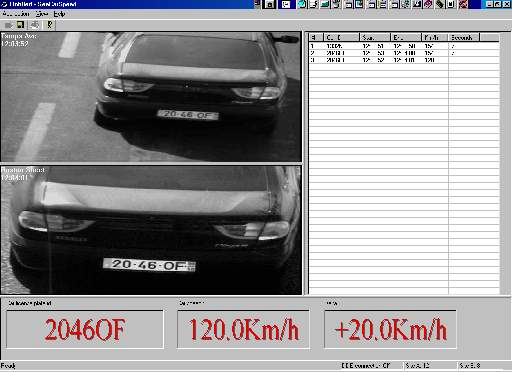
\includegraphics[width=3in]{figure/alpr.jpg}
		\caption{Automatic License Plate Recognition system takes an image of the vehicle and extracts the license plate information}
	\label{fig:alpr}
\end{figure}

However, such system requires a major upgrade in the parking lot, because it requires a completely different set of components, such as cameras, illumination, frame grabber, computer, and image-processing software. 	These equipments can be very expensive, in order to achieve a certain level of accuracy. This high cost of the system is not very appealing to the parking lot service providers. Additionally, the external effects, such as sun and headlights, and bad license plates, can severely affect the performance of the system. 

The rest of this paper will explain the system overview of our low-cost parking lot system, followed by the details of the system, evaluation, and conclusion.